%% Standard start of a latex document
\documentclass[letterpaper,12pt]{article}
%% Always use 12pt - it is much easier to read
%% Things written after '%' sign, are ignored by the latex editor - they are how to introduce comments into your .tex source
%% Anything mathematics related should be put in between '$' signs.

%% Set some names and numbers here so we can use them below
\newcommand{\name}{James Wu} %%%%%%%%%%%%%%% ---------> Change this to your name
\newcommand{\studentnumber}{92277235} %%%%%%%%%%%%%%% ---------> Change this to your student number
\newcommand{\hwnum}{4} %%%%%%%%%%%%%%% --------->  set this to the homework number

%%%%%%
%% There is a bit of stuff below which you should not have to change
%%%%%%

%% AMS mathematics packages - they contain many useful fonts and symbols.
\usepackage{amsmath, amsfonts, amssymb, bm}

%% The geometry package changes the margins to use more of the page, I suggest
%% using it because standard latex margins are chosen for articles and letters,
%% not homework.
\usepackage[paper=letterpaper,left=25mm,right=25mm,top=30mm,bottom=30mm]{geometry}
%% For details of how this package work, google the ``latex geometry documentation''.

%% Fancy headers and footers - make the document look nice
\usepackage{fancyhdr} %% for details on how this work, search-engine ``fancyhdr documentation''
\pagestyle{fancy}

\usepackage{graphicx}

\setlength{\headheight}{15pt}

%% The header
\chead{PHYS 350: Speed of Sound in a Solid} % homework number in top-centre

%% The footer
\cfoot{Page \thepage} % page in middle

%% These put horizontal lines between the main text and header and footer.
\renewcommand{\headrulewidth}{0.4pt}
\renewcommand{\footrulewidth}{0.4pt}
%%%

%%%%%%
%% The above stuff is the same as the first template, but now we are starting to prove things, so we'd like to have a
%% good proof environment that gives us nice formatting and a little square at the end.
%% We'd also like a nice Result environment that prints that up nicely too.
%% Thankfully this exists in latex in the amsthm package
\usepackage{amsthm}
\newtheorem*{thm}{Theorem}
%% This creates a new theorem-like environment called "result", that will be titled "Result".
%% See below for examples of how to use this.
%%%%%%
\usepackage{enumitem}
%% This package allows us to make nice ordered lists with numbers, letters or roman numerals

\usepackage{titlesec}
\titlespacing*{\subsection}{0pt}{0pt}{3.0ex}
\titlespacing*{\subsubsection}{0pt}{3.0ex}{0.5ex}

\usepackage[hang,flushmargin]{footmisc}

\setlength{\parindent}{0em}
\setlength{\parskip}{0.5em}

\allowdisplaybreaks

\usepackage{empheq}

\usepackage{sectsty}
\usepackage{subcaption}

\newcommand*\wfbox[1]{\fbox{\hspace{0.4em}#1\hspace{0.4em}}}

%% Useful commands
\renewcommand*{\qed}{\hfill\ensuremath{\square}}

\newcommand*{\uvec}[1]{\hat{\bm{#1}}}

\newcommand*{\deriv}[2]{\frac{d #1}{d #2}}
\newcommand*{\pderiv}[2]{\frac{\partial #1}{\partial #2}}
\newcommand*{\nderiv}[3]{\frac{d^{#3} #1}{d #2^{#3}}}
\newcommand*{\npderiv}[3]{\frac{\partial^{#3} #1}{\partial #2^{#3}}}
\newcommand*{\divg}[1]{\nabla \cdot \mathbf{#1}}

\newcommand*{\abs}[1]{\left| #1 \right|}
\newcommand*{\norm}[1]{\abs{\abs{\mathbf{#1}}}}

\newcommand*{\ev}[1]{\left<#1\right>}

\renewcommand*{\Re}[1]{\text{Re}\left(#1\right)}
\renewcommand*{\Im}[1]{\text{Im}\left(#1\right)}

\newcommand*{\qimg}[2]{\\ \begin{center}\includegraphics[scale=#1]{#2}\end{center}}

\newcommand*{\Arg}[1]{\text{Arg}\left(#1\right)}

\newcommand*{\Log}[1]{\text{Log}\left(#1\right)}

%%

\begin{document}

\begin{center}
    \subsection*{Speed of Sound in a Solid with Lagrangian Mechanics}
    James Wu, \quad 92277235
\end{center}

\begin{flushleft}

    \subsubsection*{Introduction}
    In this problem we derive an expression for the longitudinal speed of sound in a homogeneous isotropic elastic solid by modelling the solid as a three-dimensional cubic lattice. We first determine the speed of sound in terms of microscopic parameters of the material; subsequently we shall express the speed of sound in macroscopic material properties. For simplicity, we consider the case of a rectangular prism.

    \subsubsection*{Part I}
    Consider a solid rectangular prism of dimensions $a \times b \times c$ at rest. We tie our inertial reference frame to a corner of the prism with axes along those of the prism as shown in \textbf{Figure~\ref{fig:I1}}.
    \begin{figure}[h]
        \centering
        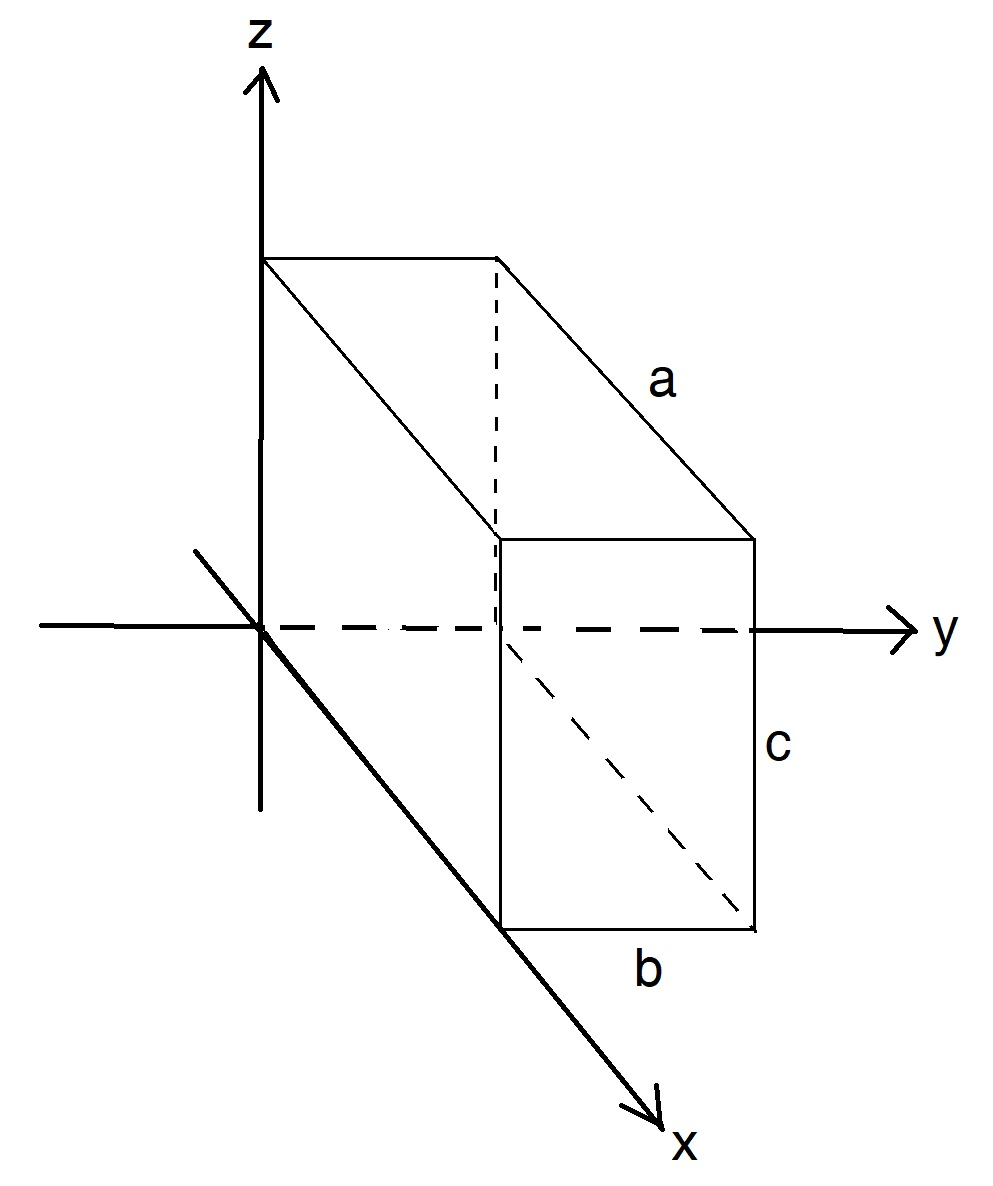
\includegraphics[scale=0.8]{images/i1.jpg}
        \caption{Sketch of the solid prism and our inertial reference frame for \textbf{Part I}. The solid is of side lengths $a$, $b$, and $c$ along the $x$-, $y$-, and $z$-axes, respectively.}
        \label{fig:I1}
    \end{figure}
    We may model this solid prism as a $M \times N \times P$ cubic lattice of point masses, each with mass $m$. These point masses represent the solid's atoms. This is illustrated in \textbf{Figure~\ref{fig:I2}}.
    \begin{figure}[h]
        \centering
        \begin{subfigure}[b]{0.6\textwidth}
            \includegraphics[width=\textwidth]{images/I2.jpg}
            \caption{}
            \label{fig:I2}
        \end{subfigure}
        \quad
        \begin{subfigure}[b]{0.3\textwidth}
            \includegraphics[width=\textwidth]{images/I3.jpg}
            \caption{}
            \label{fig:I3}
        \end{subfigure}
        \caption{(a) Sketch of the crystal lattice projected on the $xy$-plane. The black dots represent atoms; each atom in the lattice is spaced out by a distance $l_0$ at equilibrium. In total there are $M$, $N$, and $P$ atoms along the $x$-, $y$-, and $z$-axes, respectively. Although this is not depicted, this lattice repeats similarly along the $z$-axis. (b) Sketch of the interaction between an interior atom (square) and its six neighbours (circles). This interaction is modelled as a spring of equilibrium length $l_0$ and spring constant $K$. It follows that these springs lie along the $x$-, $y$-, and $z$-axes (two on each).}
    \end{figure}
    The bond potential energy between two adjacent atoms experiences a local minimum at an equilibrium length $l_0$. Applying the small oscillations approximation to this stable equilibrium, we model the interaction between two adjacent atoms as a harmonic oscillator (i.e. spring) of equilibrium displacement $l_0$ and spring constant $K$. Furthermore, we take the interaction between non-adjacent atoms to be negligible. For interior (i.e. not on the solid's boundary) atoms, this is depicted in \textbf{Figure~\ref{fig:I3}} (the boundary atoms and their interactions with the external environment determine the boundary conditions; we constrain our focus to how sound propogates inside the solid). Finally, we neglect gravity throughout this problem.\newline\newline
    To get started, how many degrees of freedom in this system? What set of generalized coordinates could you use to describe this system?

    \subsubsection*{Part II}
    We may label each atom in the lattice with indices $i$, $j$, and $k$. We shall label the corner atom at the origin with $i = 1$, $j = 1$, and $k = 1$. Then our indices range over $1 \leq i \leq M$, $1 \leq j \leq N$, and $1 \leq k \leq P$. The atom adjacent in the $x$-direction to the origin corner atom, for example, would have indices $(i, j, k) = (2, 1, 1)$. Two atoms above this atom in the $z$-direction would have indices $(i, j, k) = (2, 1, 3)$, etc. We may denote the equilibrium $x$, $y$, and $z$ positions of the $(i, j, k)$ atom as $\tilde{x}_{ijk}$, $\tilde{y}_{ijk}$, and $\tilde{z}_{ijk}$, respectively. \newline\newline
    Determine $\tilde{x}_{ijk}$, $\tilde{y}_{ijk}$, and $\tilde{z}_{ijk}$ in terms of $i$, $j$, $k$, and $l_0$. What are the dimensions $a$, $b$, and $c$ of the prism in terms of $M$, $N$, $P$, and $l_0$?

\end{flushleft}

\end{document}
